\section{ShardDAG}
\label{section:shardDAG-intro}
\todoisinline{The whole description is a part section Global Sharding Protocol/Cross-shard communication ans should be integrated in it}
zkSharding employs a directed acyclic graph (DAG) architecture called the shardDAG that combines 
 protocol rules, rewards and penalties to constrain the ability of validators to manipulate the processing of transactions.

The broad steps in achieving these constraints are to\todois{let's use figre here}
\begin{enumerate}
	\item Enforce data availability of cross-shard transactions.
	\item Enforcement of data availability enables enforcement of receipt of cross-shard transactions.
	\item Enforcement of receipt of cross-shard transactions enables enforcement of ordering of cross-shard transaction processing.
	\item Enforcement of ordering constrains the ability to insert transactions partway through other transactions, constrains delaying transaction completion and guarantees eventual transaction completion.
\end{enumerate}

A key outcome of the SharDAG is the guarantee that once a block containing cross-shard transactions is included in a (valid) consensus block, then those cross-shard transactions are guaranteed to (eventually) be completed and included\todois{Actually, just processed, not necessary completed} in their destination shards. 
Therefore, all transactions are guaranteed to complete.

Figure~\ref{figure:order-example}\todois{Figure is unreadable in this format. Adiitionally, it should be aligned with the style of other figures} illustrates\todois{If it illustrates then it doesn't require so much text under it} how the shardDAG induces an order of transaction and cross-shard transaction processing. Briefly, within a shard block's subgraph, the shardDAG is used to partially order shard blocks. The partial ordering of shard blocks is then used to create a partial ordering of transactions and cross-shard transactions.

\begin{figure}
	\centering
	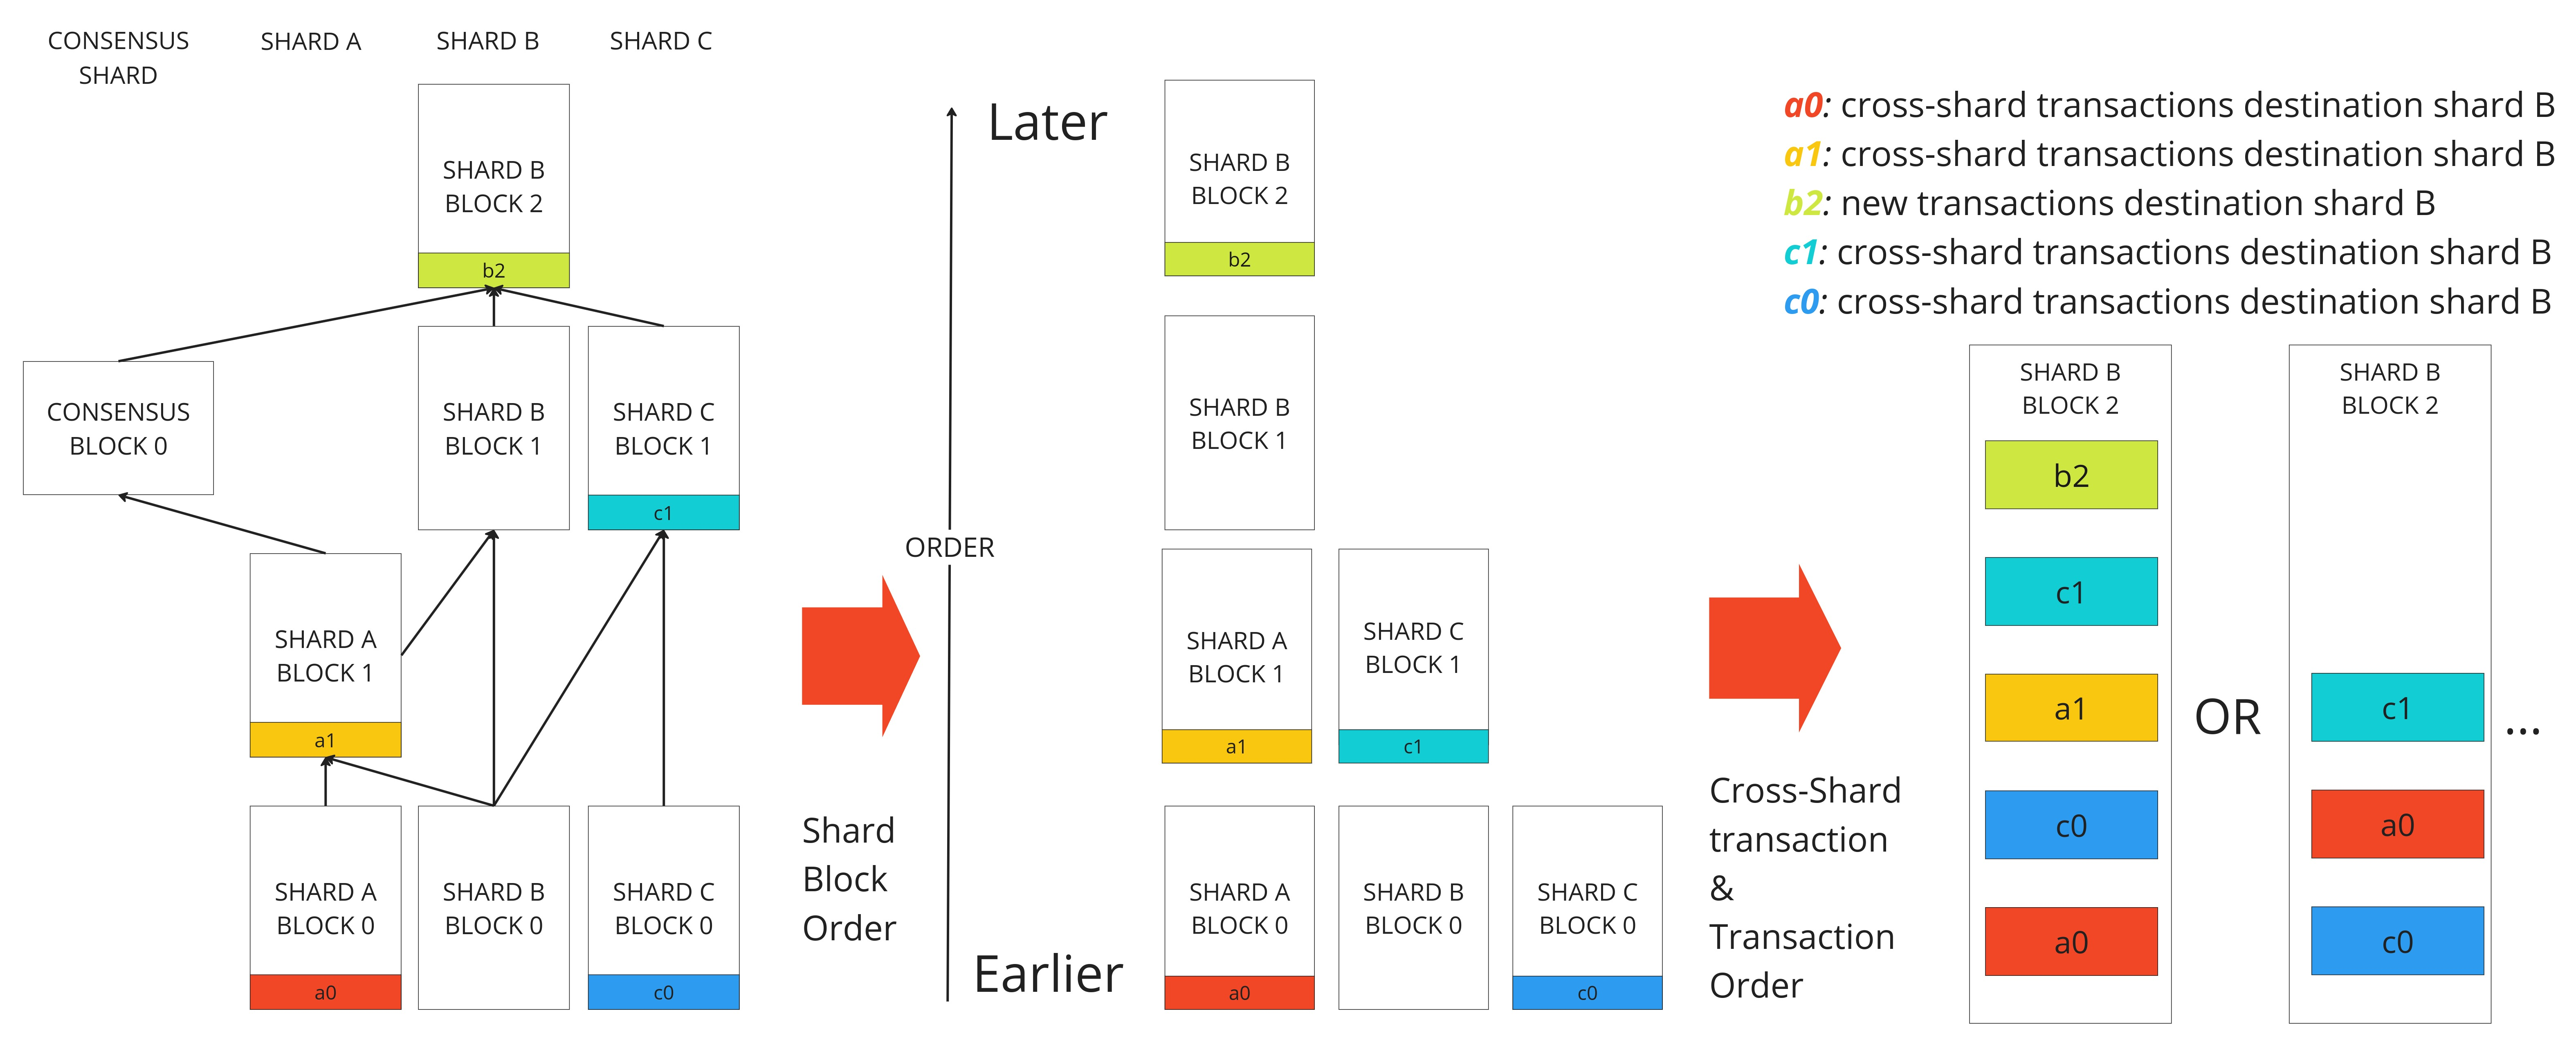
\includegraphics[width=0.8\textwidth]{figures/OrderExample.jpg}
	\caption{An example ordering of a shardDAG and its constituent cross-shard transactions, and new transactions. 
		Left: In this example shard $B$ block 2 is in the process of being created using hashes to shard $B$ block 1 and shard $C$ block 1 (dashed arrows). 
		It is assumed that all cross-shard transactions are pending (i.e. not included in shard $B$ block 1 or earlier). 
		Centre: Shard $B$ block 2’s subgraph of shard blocks are ordered. 
		Right: Two example valid orderings of cross-shard transactions are shown. 
		The orders follow the centre block ordering. 
		Shards can select the order of cross-shard transactions amongst blocks that are equally ordered. 
		However, shards are forced to process early cross-shard transactions, in particular note that the new shard $B$ transactions $b2$ cannot be included before existing cross-shard transactions. If block capacity restricts inclusion, only the lowest (earliest) cross-shard transactions are included in shard $B$ block 2. }
	\label{figure:order-example}
\end{figure}

\subsection{Shard DAG Formation}
To form a shardDAG shard blocks include
\begin{itemize}
	\item A hash to the previous (valid) shard block in the same shard, as in a typical blockchain.
	\item A set of hashes to other shards blocks in other shards.
	Up to $N-1$ hashes are allowed, where $N$ is the number of shards. 
	At most one hash per shard is allowed, and no hash can fall in the subgraph of another hash, to eliminate redundant data.
	\item a hash to a (valid) consensus block, equal to or later than the most recent consensus block already included in prior shard blocks.	
\end{itemize}
The subgraph of a shard block $b$ includes all shard blocks that can be reached starting from $b$ (including $b$ itself) by traversing edges in the shardDAG, including edges to and from consensus blocks.

An example shardDAG is illustrated in Fig.~\ref{figure:shard-formation}\todois{unreadable, requires to change style}. 
Blue lines depict the subgraph of the top left shard block, obtained by following the hash lists in each shard block header. 
The dotted red line indicates an invalid hash because the lower shard block falls in the subgraph of another hash and is therefore redundant.
The top left block must process (unprocessed) shard transactions in the order in which they appear in its subgraph.

\begin{figure}
	\centering
	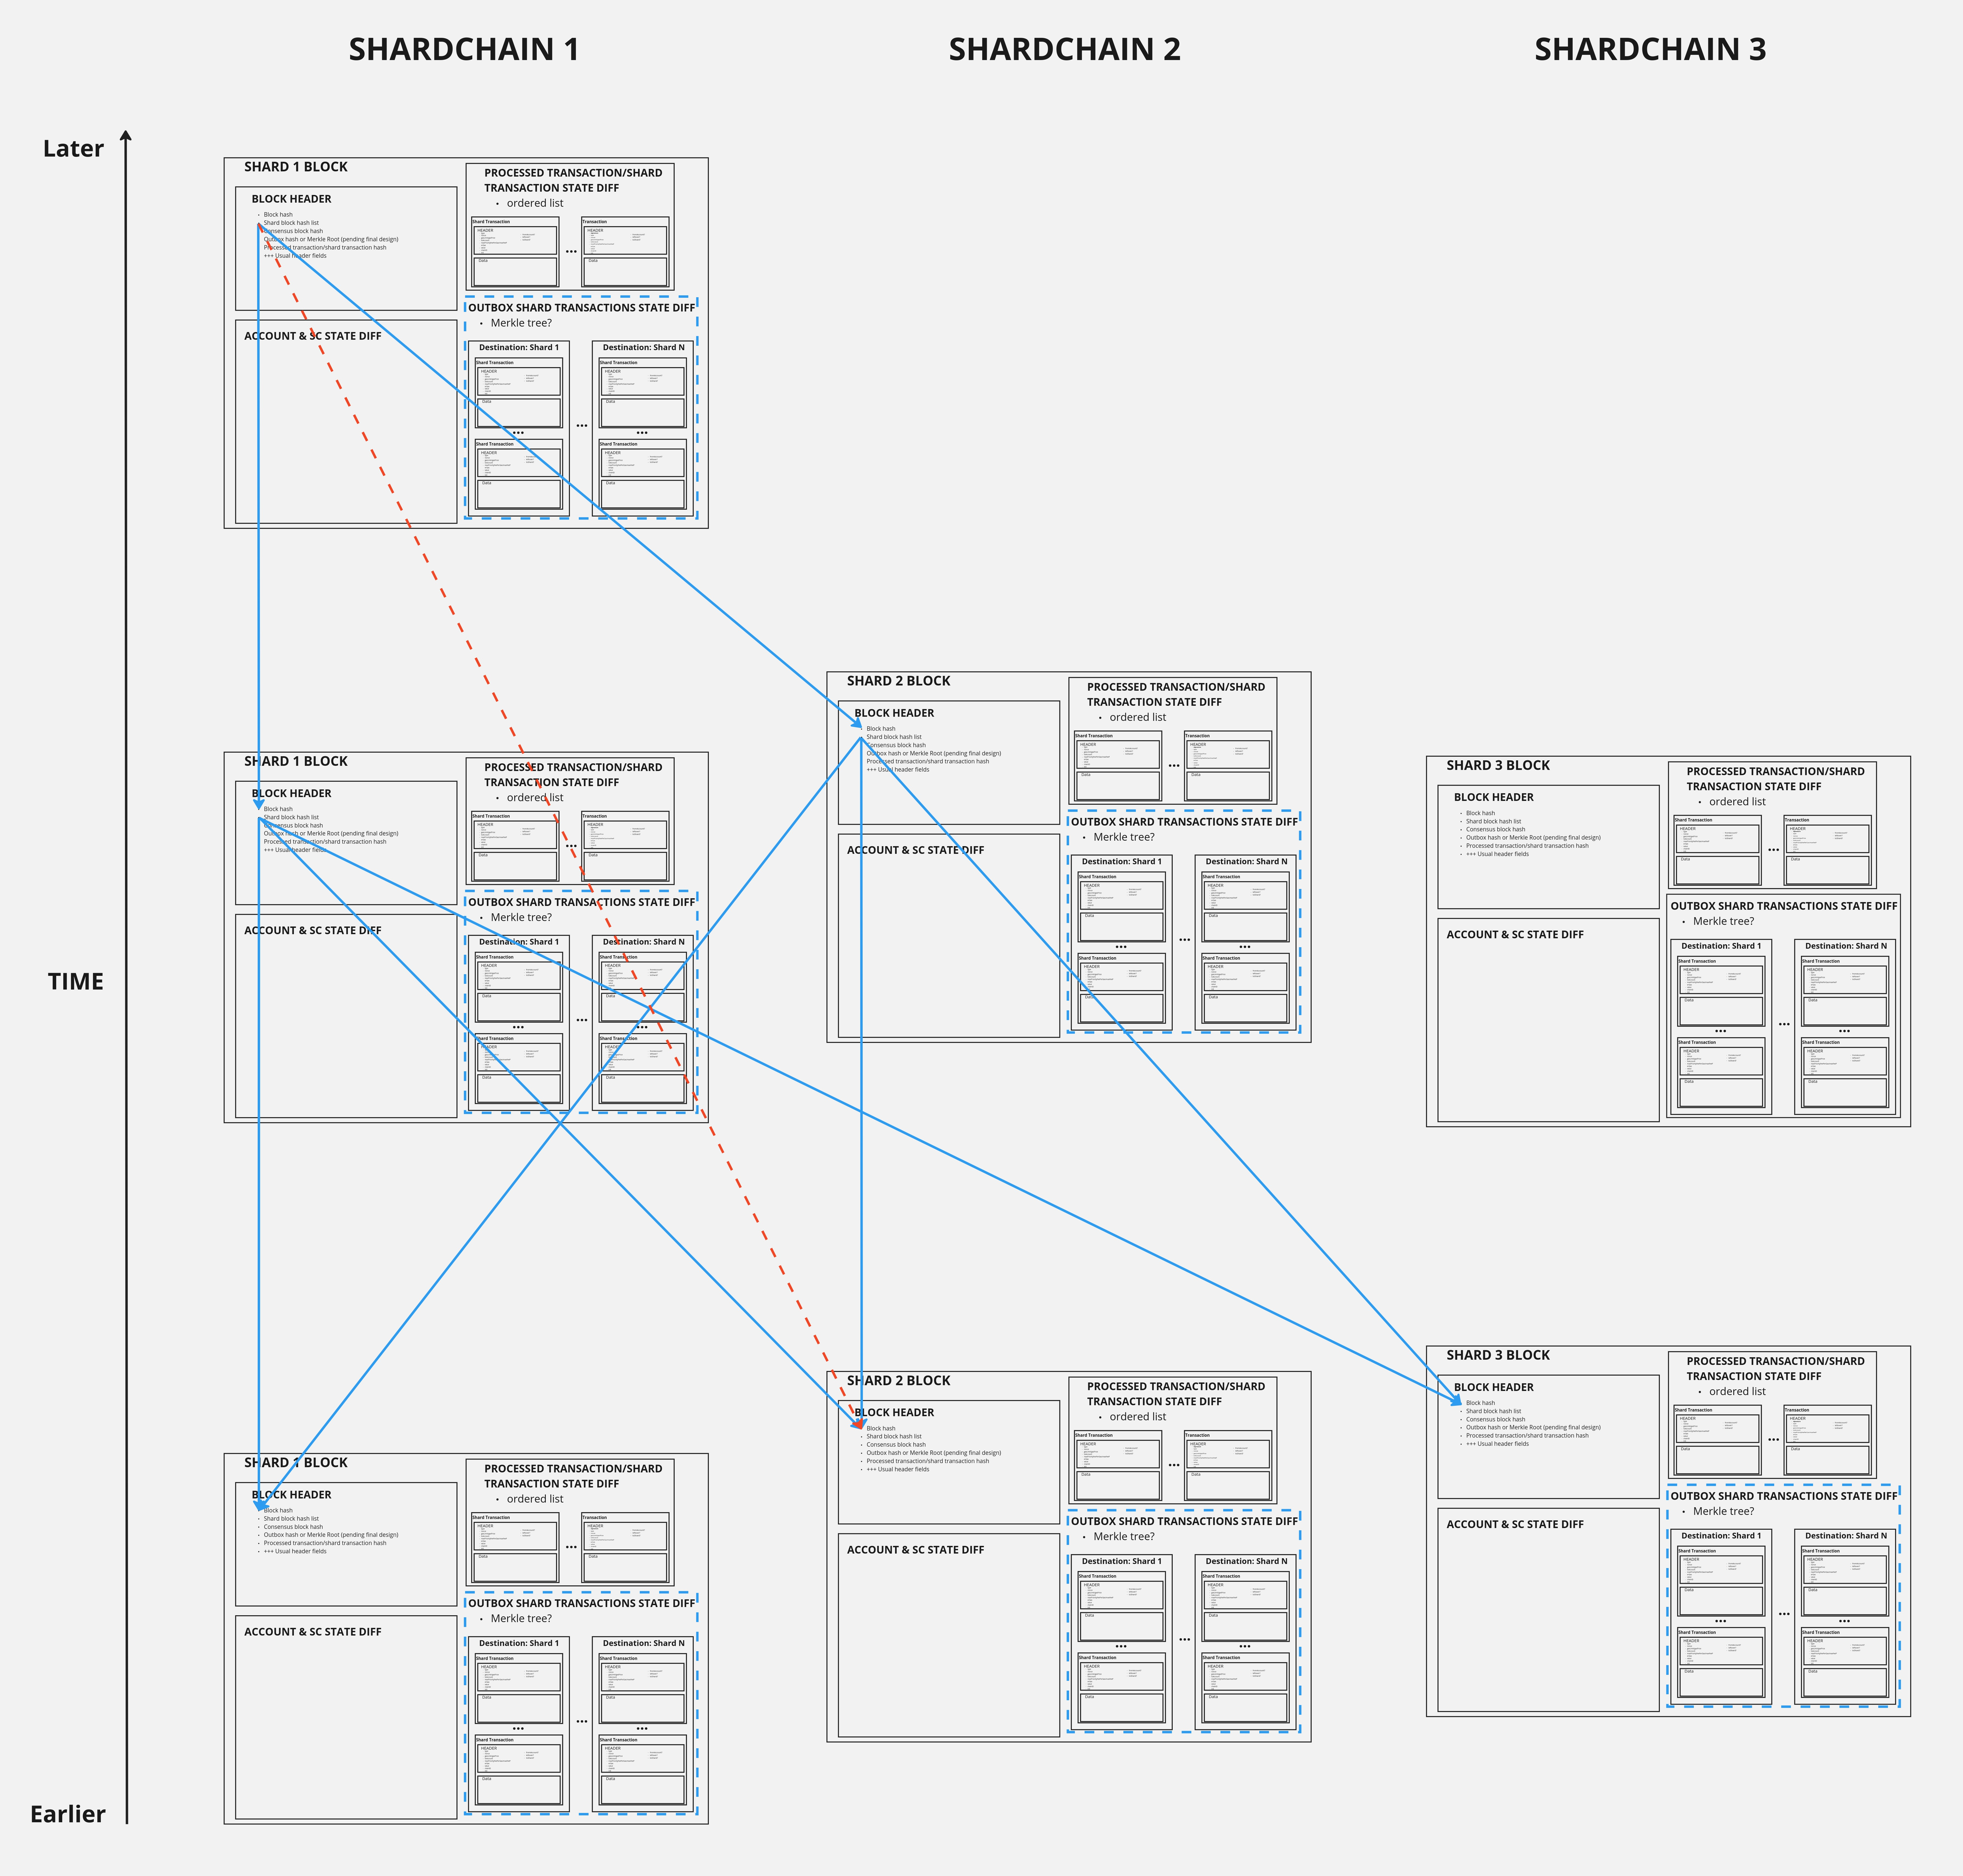
\includegraphics[width=0.8\textwidth]{figures/DetailedShardDAGEdgeRules.jpg}
	\caption{ Illustration of a shard DAG. 
		Each shard block’s header contains a list of hashes to other shard blocks (blue arrows), and well as a single hash to a consensus block (not shown). 
		The dotted red arrow indicates a hash that is not allowed, because the lower block is in the subgraph of a higher shard block, and the edge is therefore redundant. 
		For clarity not all edges between blocks are shown}
	\label{figure:shard-formation}
\end{figure}




\subsection{Block Creation}

Validators only propose and sign shard blocks that comply with the shardDAG protocol rules listed below. 
In constructing the shardDAG it is assumed that there is some maximum number of malicious shards $F$\todois{change to generic parameter}. 


\subsubsection{Valid Block Conditions}
For a given shard block $b$ to be valid, it must satisfy all the below conditions:
\begin{itemize}
	\item $[$ORDERING CONDITION$]$\todois{Change in alignment to other styling: textbb without capitalization}:\todois{Hard-readable, need better structure} For a given shard block $b$ the set $T$ of all transactions and cross-shard transactions in $b$’s subgraph (including those in $b$) are partially ordered using the Lamport timestamps $L$ of their containing block. 
	For a shard block to be valid, the shard block’s set of processed transactions $P$ must be the subset of unprocessed (in prior blocks) $T$ with smallest $L$. 
	The order in which $P$ are processed must conform to the $L$ ordering. 
	No rules apply to ordering within sets of transactions and cross-shard transactions with equal $L$, block producers are expected to (but not required to) order based on MEV. 
	$b$ must not process any cross-shard transactions that do not appear in its subgraph.
	
	\item $[$PARENT CONDITION$]$: For a given shard block $b$ with parent $a$ from the same shard block, $b$’s subgraph must contain shard blocks created by $>F$ shards that are not present in the subgraph of $a$. 
	At most one hash per shard is allowed, and no hash can fall in the subgraph of another hash, to eliminate redundant data.
	\item $[$CONSENSUS-PARENT CONDITION$]$: For a given shard block $b$ with consensus block parent $c$, there must be $X$ prior shard blocks from $b$’s shard that also have $c$ as a consensus block parent. 
	$X$ is to be chosen once relative timings of consensus and shard blocks becomes clearer.
\end{itemize}
The purpose of the parent and consensus-parent conditions are to force shards to acknowledge the receipt of shard block headers and outboxes of cross-shard transactions.
The purpose of the ordering condition is to force shards to obey a clearly defined method for ordering the processing of transactions and cross-shard transaction that each shard has acknowledged receiving. 
This ordering of transaction and cross-shard transaction processing can be verified and penalties can be applied for breaches of correct ordering.

The following is a central concept in the function of the shardDAG.
When shard $A$ creates a shard block that includes the hash of another shard block $H$, this inclusion acts as an acknowledgement that shard $A$ has received the headers and outboxes of cross-shard transactions for $H$ and $H$’s entire subgraph in the shardDAG, up to a limit at which it has been established that this data is no longer required, see Sec.~\ref{section:shardDAG-data-storage}.

An honest validator should not sign a consensus block until it possess the shard block headers and outboxes of cross-shard transactions contained within the consensus block.
If a shard block includes a consensus block, or a shard block in its shard block's subgraph, but the creator does not possess the required data, then the shard block risks processing transactions and cross-shard transactions in the incorrect order and therefore incurring penalties, and potentially initiating a rollback.

 
\subsubsection{Shard Block Finalisation Condition}
\label{section:shard-block-finalisation}
\todoisinline{It's not the only finzalization condition, but the one enorced by ShardDAG, underline that fact}
The consensus shard incorporates the shardDAG by including sets of shard blocks in each consensus block. 
Let $D$ be the subset of the shardDAG that has been included in consensus blocks. Before a shard block $b\in D$ can be finalised within the consensus chain it must satisfy the following condition
\begin{itemize}
	\item $[$CHILD CONDITION$]$: Within $D$, there must be $>F$ shards that have one or more blocks whose subgraph contains $b$.
\end{itemize}
The purpose of this child condition is to force shards to distribute their shard block headers and outboxes of cross-shard transactions {\it before} they are included in a consensus block, thus constraining the ability of shards to withhold and delay cross-shard transaction processing.



\subsubsection{Local ShardDAG Construction}
Each validator constructs its own local shardDAG as follows
\begin{itemize}
	\item Newly received shard blocks undergo basic validity checks, like checking signatures, checking for $>F$ shard block hashes etc.
	\item Shard blocks that meet the above basic validity checks are held in a buffer.
	\item Shard blocks are moved from the buffer to the shardDAG i) when a shard block in a buffer has all of its parents (its shard block hashes) already included in the DAG, and ii) when the validator has received and verified the shard block's outbox shard transactions.	
\end{itemize} 
The above ensures that the local shardDAG only includes valid shard blocks and the local shardDAG is not missing any shard blocks (no `holes' in the shardDAG where edges do not have a block on both ends).



\subsection{Data Communication}
\todoisinline{the section can be skipped in the doc for the sake of calrity}
Push messaging describes messaging in which the sender of data initiates communication. 
When a new shard block is finalised at the shard chain level (signed by at least quorum validators in a shard), validators within that shard broadcast the shard block header and outbox shard transactions to all validators using a push messaging system. This ensures other shards can include newly created shard blocks in their own subgraphs as soon as possible, and in return allows newly created shard blocks to be finalised according to the child condition in Sec.~\ref{section:shard-block-finalisation}.

Pull messaging describes messaging in which the receiver of data initiates communication. In zkSharding there are a few main scenarios when pull messaging should be used.

\begin{itemize}
	\item A validator participating in the consensus chain receives a consensus block proposal containing the hash of a shard block for which it does not possess the shard block data. 
	Before signing the consensus block, the validator must first request the shard block header, and cross-shard transaction outbox, before verifying it and deciding whether to sign the consensus block, or not.
	The above also applies to validators participating in shard consensus, but additionally requires entire shard block data before signing a shard block.
	\item When a validator becomes the consensus chain leader and must build a consensus block for proposal, but the validator suspects that it may not possess blocks near the head of some shardchain(s), perhaps because a long time has elapsed since the validator last received a new shard block from some shard(s). 
	In this case, the lead validator can request this data using pull messaging.
	The above also applies to validators participating in local shard consensus. 
	Further, if a lead validator possesses a shard block $b$ and its outbox shard transactions, it may request any missing parts of $b$’s subgraph, so that the leader can include $b$ in its new shard block.
\end{itemize}

The need here for pull messaging differs from non-sharded blockchains. 
In non-sharded blockchains if validators are not synced then they must request (pull) data from the network to catch up to the head before they can sign or propose new blocks. 
However, most validators must be synced at the head of the chain otherwise new (valid) blocks cannot be produced. 
If insufficient validators are not synced to the head, then block production is delayed, this self-limiting design means that most validators tend to remain synced to the head of the chain.

The zkSharding blockchain contains many individual shard chains, each with its own head shard block. 
Creation of new shard blocks only requires the shard subset of validators to be synced to the head of the shard chain. 
Thus, unlike a non-sharded blockchain it is possible for a shard chain to extend while many validators that are not part of its validating set fall behind.

For scalability reasons when creating a new consensus block it is not efficient for a consensus block proposer to initiate a push distribution of all shard blocks included in its consensus block, especially when all validators should already posses most of these shard blocks through shard-level push messaging.
Instead, upon receiving a new consensus block each validator should identify any shard blocks it does not possess and request them using pull messaging. 
This can be aided by the shardDAG to identify which shards attest to possessing each missing shard block and therefore where requests should be sent.

To summarise the above, push messaging should be used to deliver most shard block and cross-shard transaction data because this data needs to be distributed widely within the network with low latency. However, pull messaging is used in (hopefully) relatively few instances where push messaging has not (yet) delivered necessary data.


\subsection{Data Storage}
\label{section:shardDAG-data-storage}
\todoisinline{the section can be skipped in the doc for the sake of calrity}
Validators store all shard block data for their own shard.
Validators can delete shard block outboxes of cross-shard transactions once they have been processed by their destinations shards and ZK finalised, after which they are no longer required.
An efficient process for determining when data is no longer required is described in App.~\ref{appendix:shardDAG-deletion}.


%\subsection{Detecting Invalid Behaviour}
%+++TODO

%\subsection{Rewards and Penalties}
%+++TODO
